\subsection{Description}
To execute the main objective, the alloy model depicts the following logics:
\begin{itemize}
\item There are two users individual and third party.
\item Individual has one wearable device that gives Location and Health vitals of that Individual.
\item Third Party can make Group Request and Individual Request.
\item When the health status of an Individual is below the threshold value, the critical condition is True.
\item The ambulance gets the details of the individual whose critical condition is true.
\item The details of the individual is connected to the ambulance that is near to the individual location.
\item An organizer is a Third Party who organizes the Event.
\item An Athlete is an Individual who joins the Event.
\item A spectator can be both Individual and Third party who watches the event.
\item An event has date, time, and location.
\end{itemize}
\subsection{Alloy code}
\begin{figure}[H]
	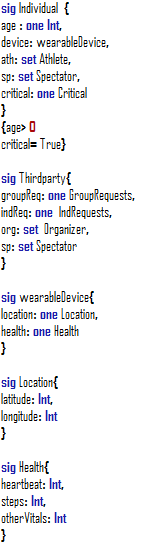
\includegraphics[width=5cm,height=18cm]{./Alloy/sig1.PNG}
\end{figure}
\begin{figure}[H]	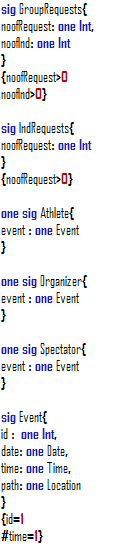
\includegraphics[width=5cm,height=18cm]{./Alloy/sig2.PNG}
\end{figure}
\begin{figure}[H]	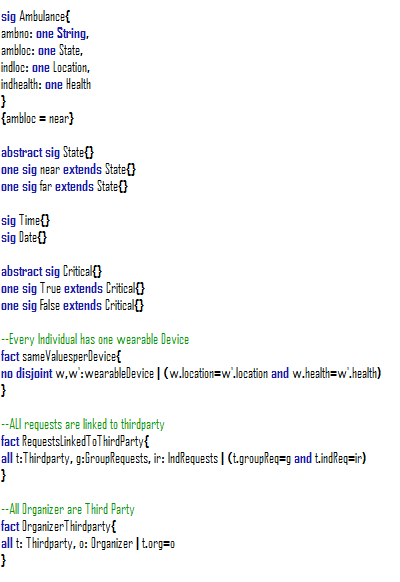
\includegraphics[width=\linewidth]{./Alloy/sig3+fact1.PNG}
\end{figure}
\begin{figure}[H]	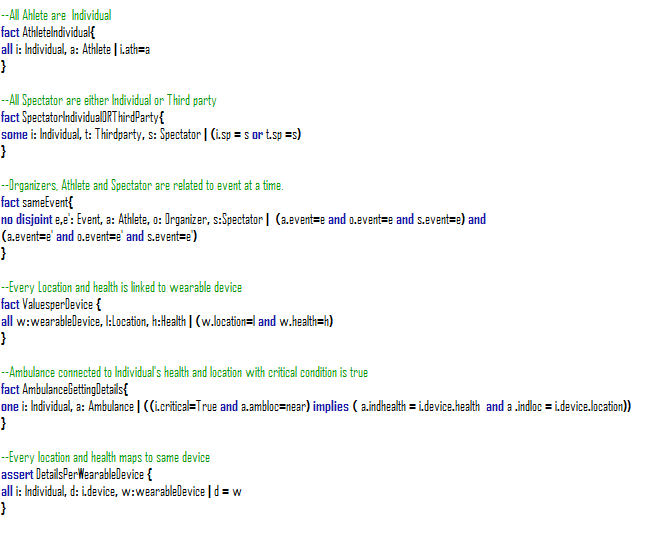
\includegraphics[width=16cm,height=18cm]{./Alloy/fact2+assert1.PNG}
\end{figure}
\begin{figure}[H]	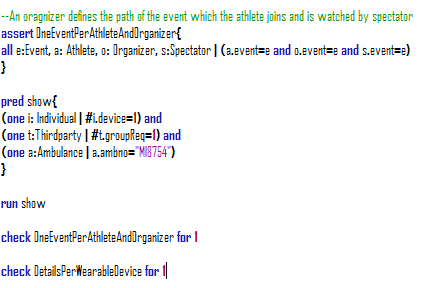
\includegraphics[width=16cm,height=12cm]{./Alloy/assert2+pred.PNG}
\end{figure}
\subsection{Result}
\begin{figure}[H]	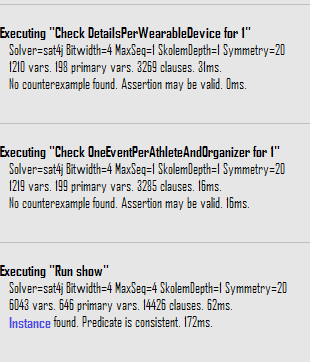
\includegraphics[width=\linewidth]{./Alloy/Result.PNG}
\end{figure}
\subsection{Alloy Model}
\begin{figure}[H]	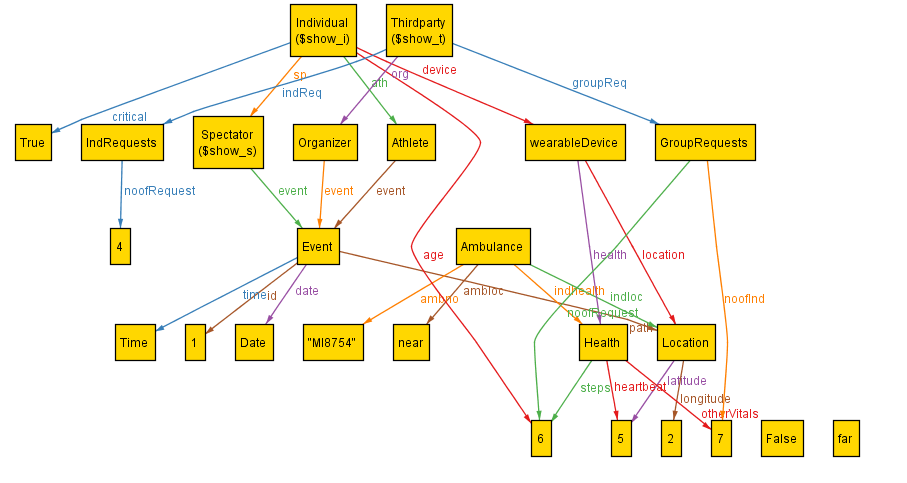
\includegraphics[width=\linewidth]{./Alloy/Final_model.PNG}
\end{figure}